\section{Diffuse Reflection of Beam Solar and Sky Solar Radiation}\label{diffuse-reflection-of-beam-solar-and-sky-solar-radiation}

A ray-tracing method is used to calculate beam solar and sky solar radiation that is diffusely reflected onto each of a building's exterior surfaces (walls, roofs, windows and doors), called here ``receiving surfaces.'' The calculation begins by generating a set of rays proceeding into the outward hemisphere at each receiving point on a receiving surface. Then it determinines whether each ray hits the sky, ground or an obstruction. The radiance at the hit point from reflection of incident beam or sky solar is determined and the contribution of this radiance to the receiving surface is calculated, added to the contribution from other hit points, and averaged over the receiving points. Separate calculations are done for beam-to-diffuse and sky solar reflection from all obstructions and beam-to-diffuse and sky solar reflection from the ground. (For beam-to-beam reflection see ``Beam Solar Radiation Specularly Reflected from Obstructions,'' below.)

\subsection{Receiving points}\label{receiving-points}

An \emph{N}-sided surface is assigned \emph{N} receiving points with the following coordinates, expressed in terms of the surface vertex coordinates:

\begin{equation}
{P_{ij}} = \sum\limits_{k = 1}^N {{a_{ki}}{v_{kj}},{\rm{  }}i = 1,3;{\rm{  }}j = 1,3}
\end{equation}

where

\emph{P\(_{ij}\) = j\(^{th}\)} coordinate of the i\(^{th}\) receiving point

\emph{v\(_{kj}\)} = j\(^{th}\) coordinate of the \emph{k\(^{th}\)} surface vertex

If \emph{N} = 3:~ \emph{a\(_{kj}\)} = 3/5 if \emph{k} = \emph{i};~\emph{a\(_{kj}\)} = 1/5 otherwise

If \emph{N} \textgreater{} 3:~ \emph{a\(_{kj}\)} = \(\frac{{N + 1}}{{2N}}\) ~if \emph{k} = \emph{i};~\emph{a\(_{kj}\)} = \(\frac{1}{{2N}}\) ~otherwise

For example, for a vertical 3m by 5m rectangle with vertices (0,0,3), (0,0,0), (5,0,0) and (5,0,3), this expression gives receiving points at (1.25,0,2.25), (1.25,0,0.75), (3.75,0,0.75) and (3.75,0,2.25), as shown in Figure~\ref{fig:vertical-rectangular-exterior-heat-transfer}.

\begin{figure}[hbtp] % fig 53
\centering

\includegraphics[width=0.9\textwidth, height=0.9\textheight, keepaspectratio=true]{media/image676.png}
\caption{Vertical rectangular exterior heat transfer surface showing location of receiving points for calculating incident solar radiation reflected from obstructions. \protect \label{fig:vertical-rectangular-exterior-heat-transfer}}
\end{figure}

\subsection{Rays}\label{rays}

A total of 90 rays are sent out into the exterior hemisphere surrounding each receiving point. An upgoing ray may hit an obstruction or the sky. A downgoing ray may hit an obstruction or the ground. See Figure~\ref{fig:two-dimensional-schematic-showing-rays-going}.

In subroutine InitSolReflRecSurf, the following is determined for each ray, \emph{i,}:

1.~~~~Unit vector in direction of ray

2.~~~~Cosine of angle between ray and plane of receiving surface (\(\cos {\alpha_i}\) )

3.~~~~Element of solid angle associated with ray (\(d{\Omega_i}\) )

4.~~~~If the ray hits one or more obstructions, the coordinates of the hit point on the obstruction nearest the receiving point

5.~~~~For the surface containing the hit point: the surface number, the solar reflectance (\({\rho_{obs,i}}\) if an obstruction), and the surface unit vector at the hit point pointing into the hemisphere containing the receiving point

6.~~~~If the ray is downgoing and hits the ground, the coordinates of the ground hit point

7.~~~~Distance from receiving point to hit point

\begin{figure}[hbtp] % fig 54
\centering
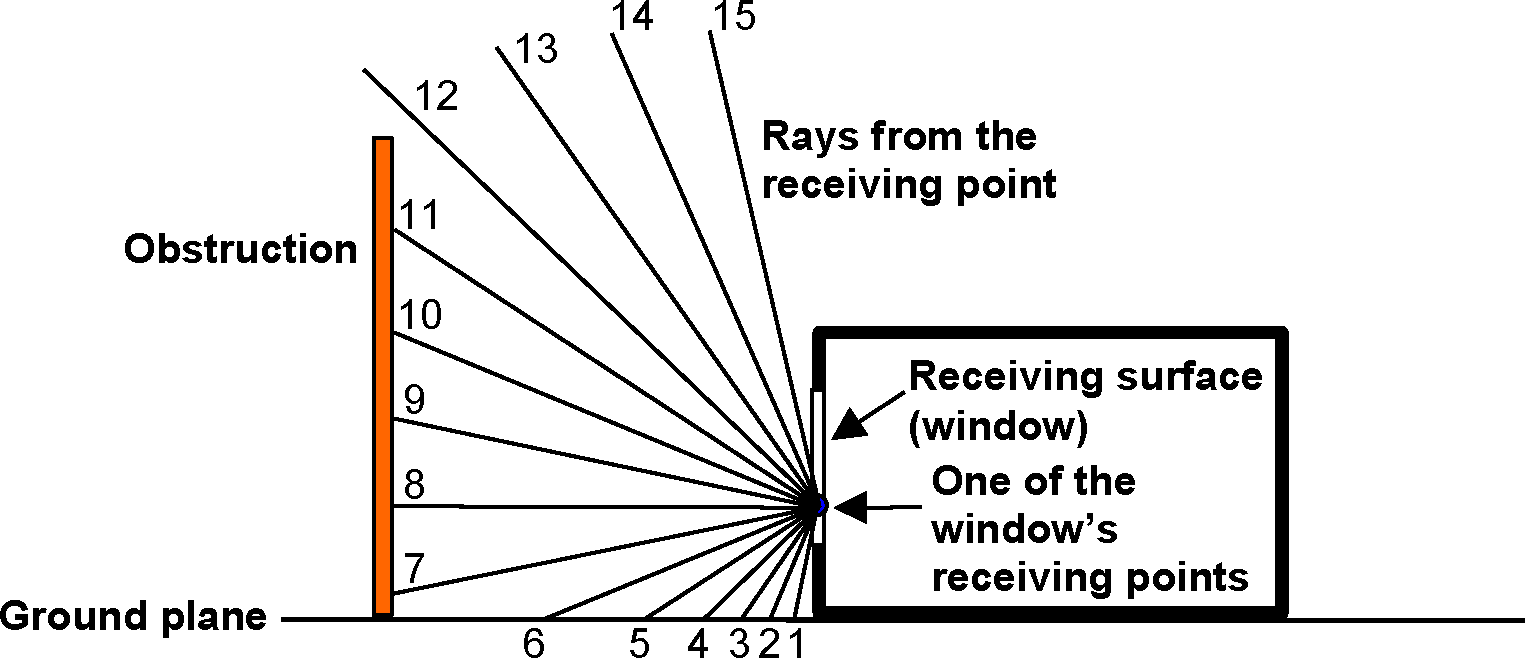
\includegraphics[width=0.9\textwidth, height=0.9\textheight, keepaspectratio=true]{media/image680.png}
\caption{Two-dimensional schematic showing rays going outward from a point on a receiving surface. Rays 1-6 hit the ground, rays 7-11 hit an obstruction, and rays 12-15 hit the sky. \protect \label{fig:two-dimensional-schematic-showing-rays-going}}
\end{figure}

\subsection{Sky Solar Radiation Diffusely Reflected from Obstructions}\label{sky-solar-radiation-diffusely-reflected-from-obstructions}

The factor for reflection of sky radiation from obstructions onto a receiving surface is calculated in subroutine CalcSkySolDiffuseReflFactors. It is given by:

\begin{equation}
\begin{array}{l}{\rm{ReflFacSkySolObs(RecSurfNum)}} = \\\frac{1}{{{N_{rec}}}}\sum\limits_1^{{N_{rec}}} {\sum\limits_{i = 1}^{{N_{ray}}} {Hi{t_{obs,i}}ViewFacSk{y_{obs,i}}DifShdgRatioIsoSk{y_{obs,i}}{\rho_{obs,i}}\cos {\alpha_i}/\pi } } \end{array}
\end{equation}

where

RecSurfNum is the receiving surface number,

\({N_{rec}}\) is the number of receiving points,

\({N_{ray}}\) is the number of rays,

``\emph{obs,i}'' denotes the obstruction hit by ray \emph{i},

\emph{Hit\(_{obs,i}\)} = 1 if ray \emph{i} hits an obstruction, = 0 otherwise,

\emph{ViewFacSky\(_{obs,i}\)} = unobstructed sky view factor of the obstruction = \((1 + \cos til{t_{obs}})/2\) ,

\emph{DifShdgRatioIsoSky\(_{obs,i}\)} = (obstructed sky irradiance on obstruction)/(unobstructed sky irradiance on obstruction)

In this equation, the product \emph{ViewFacSky*DifShdgRatioIsoSky} is the sky irradiance at the hit point divided by the horizontal sky irradiance taking into account shadowing of sky diffuse radiation on the obstruction by other obstructions, and assuming that the radiance of the sky is uniform. Note that we ignore secondary reflections here and in the following sections. In the present case this means that the irradiance at the hit point due to reflection of sky radiation from the ground or from other obstructions is not considered.

The above reflection factor is used in the timestep calculation to find the irradiance on a receiving surface due to sky radiation reflected from obstructions:

\begin{equation}
QRadSWOutIncSkyDiffReflObs(RecSurfNum) = DifSolarRad * ReflFacSkySolObs(RecSurfNum) (W/m^{2})
\end{equation}

where \emph{DifSolarRad} is the horizontal sky irradiance on an unobstructed horizontal plane (W/m\(^{2}\)).

\subsection{Sky Solar Radiation Diffusely Reflected from the Ground}\label{sky-solar-radiation-diffusely-reflected-from-the-ground}

If a downgoing ray from a receiving point hits the ground (for example, rays 1-6 in Figure~\ref{fig:two-dimensional-schematic-showing-rays-going}), the program calculates the radiance at the ground hit point due to sky diffuse solar reaching that point. To do this, rays are sent upward from the ground hit point and it is determined which of these rays are unobstructed and so go to the sky (for example, rays 6-10 in Figure~\ref{fig:two-dimensional-schematic-showing-rays-going-001}). For this calculation it is assumed that the radiance of the sky is uniform.

\begin{figure}[hbtp] % fig 55
\centering
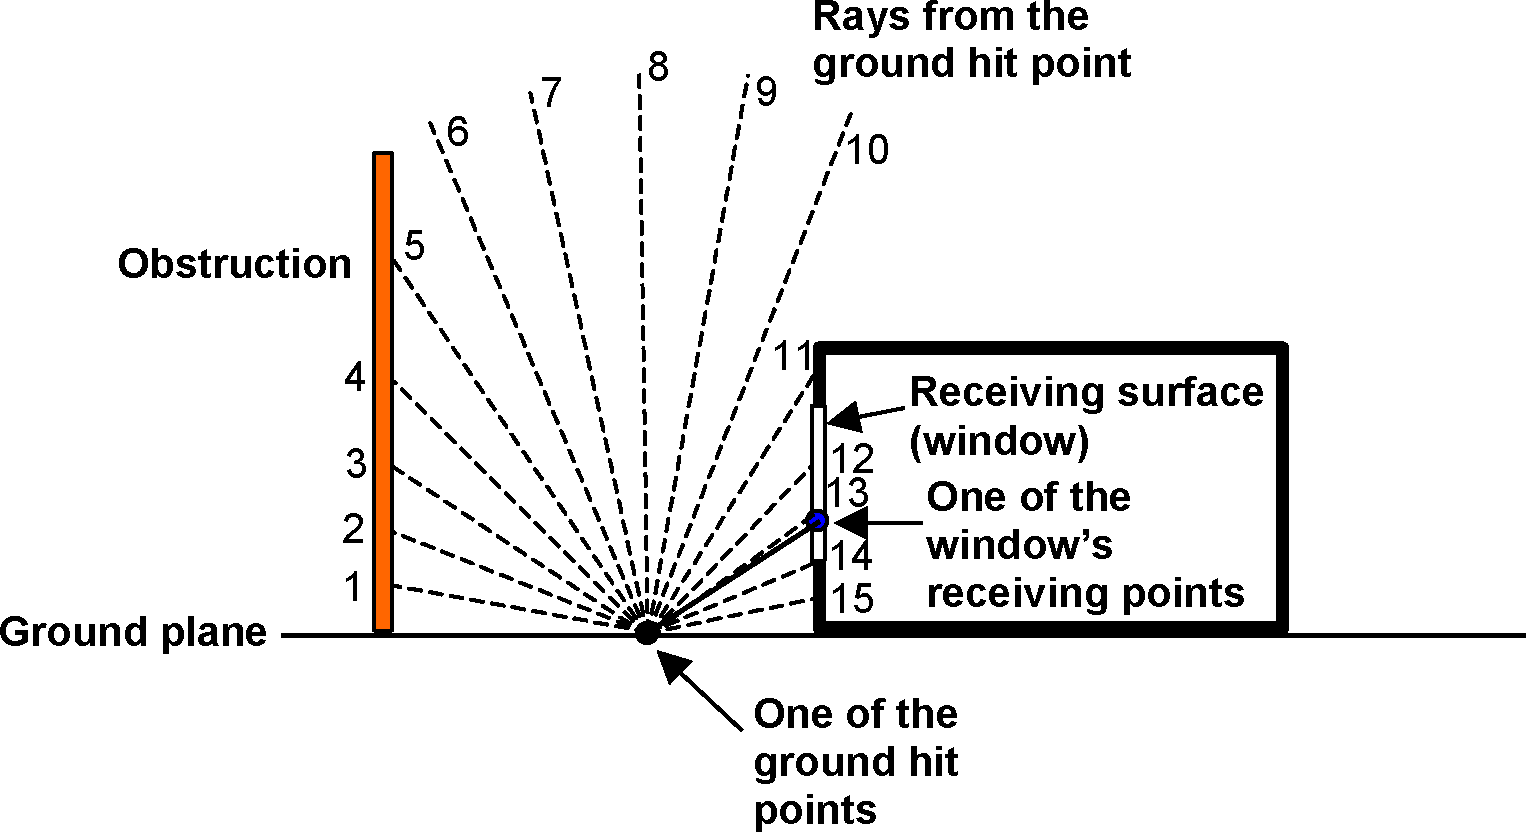
\includegraphics[width=0.9\textwidth, height=0.9\textheight, keepaspectratio=true]{media/image685.png}
\caption{Two-dimensional schematic showing rays going upward from a ground hit point. \protect \label{fig:two-dimensional-schematic-showing-rays-going-001}}
\end{figure}

The factor for reflection of sky radiation from the ground onto a receiving surface is calculated in subroutine CalcSkySolDiffuseReflFactors. It is given by:

\begin{equation}
\begin{array}{l}
{\rm{ReflFacSkySolGnd(RecSurfNum)}} = \\\frac{1}{{{N_{rec}}}}\sum\limits_1^{{N_{rec}}} {\sum\limits_{i = 1}^{{N_{ray}}} {\left[ {(Hi{t_{gnd,i}}d{\Omega_i}\cos {\alpha_i}/\pi )\sum\limits_{j(i)}^{{N_{ray}}} {Hi{t_{sky,j(i)}}\cos {\alpha_{j(i)}}d{\Omega_{j(i)}}/\pi } } \right]} }
\end{array}
\end{equation}

where

\emph{\(j(i)\) ~}~denotes an upgoing ray from the ground point hit by ray \emph{i}from the receiving point,

\emph{Hit\(_{skyj(i)}\)} = 1 if ray \emph{\(j(i)\)} hits the sky, = 0 otherwise,

\({\alpha_{j(i)}}\) is the angle of incidence of ray \(j(i)\) with respect to the ground plane,

\(d{\Omega_{j(i)}}\) is the solid angle element associated with ray \(j(i)\) .

This factor is used in the timestep calculation to find the irradiance on a receiving surface due to sky radiation reflected from the ground:

\begin{equation}
QRadSWOutIncSkyDiffReflGnd(RecSurfNum) = DifSolarRad * {\rho_{gnd}} * ReflFacSkySolGnd(RecSurfNum)~ (W/m^{2})
\end{equation}

where \({\rho_{gnd}}\) is the solar reflectance of the ground, which is assumed to be uniform over the ground plane but may vary monthly (because of snow cover, for example).

\subsection{Beam Solar Radiation Diffusely Reflected from Obstructions}\label{beam-solar-radiation-diffusely-reflected-from-obstructions}

This calculation is similar to that for sky solar reflected from obstructions. However, to find the radiance at a hit point on an obstruction a line is drawn from the hit point to center of the sun. From this line it is determined (1) if there is an obstruction between the hit point and the sun, in which case it is assumed that no beam solar reaches the hit point; and (2) if beam solar does reach the hit point, what the the solar angle of incidence at that point is.

The calculation is done for the hourly sun positions on each of the design days. It is also done for hourly sun positions on selected days during the weather file run period (the same days for which the shadowing calculations are done).

The factor for diffuse reflection of beam solar radiation from obstructions onto a receiving surface is calculated in subroutine CalcBeamSolDiffuseReflFactors. It is given by:

{\scriptsize
\begin{equation}
{\rm{ReflFacBmToDiffSolObs(RecSurfNum,IHr)}} = \frac{1}{{{N_{rec}}}}\sum\limits_1^{{N_{rec}}} {\sum\limits_{i = 1}^{{N_{ray}}} {Hi{t_{obs,i}}Hi{t_{obs,i,sun}}d{\Omega_i}\cos {\alpha_i}{\rho_{obs,i}}\cos {\alpha_{sun,obs,i}}} }
\end{equation}}

where

\emph{IHr} = hour number

\(Hi{t_{obs,i}}\) = 1 if ray \emph{i} from the receiving point hits an obstruction, = 0 otherwise,

\(Hi{t_{obs,i,sun}}\) = 1 if the line from ray \emph{i}'s hit point to the sun is unobstructed, = 0 otherwise,

\({\alpha_{sun,obs,i}}\) is the angle of incidence of the sun on the obstruction.

This factor is used in the timestep calculation to find the diffuse irradiance on a receiving surface due to beam solar diffusely reflected from obstructions:

\begin{equation}
\begin{split}
QRadSWOutIncBmToDiffReflObs(RecSurfNum) = BeamSolarRad \\
* (WeightNow * ReflFacBmToDiffSolObs(RecSurfNum,HourOfDay) \\
+ WeightPreviousHour * ReflFacBmToDiffSolObs(RecSurfNum,PreviousHour))
\end{split}
\end{equation}

where \emph{BeamSolarRad} is the timestep value of beam normal solar intensity \(W/{m^2}\), and \emph{WeightNow} and \emph{WeightPreviousHour} are time-averaging factors.

\subsection{Beam Solar Radiation Diffusely Reflected from the Ground}\label{beam-solar-radiation-diffusely-reflected-from-the-ground}

This calculation is the same as that for beam solar diffusely reflected from obstructions except that only rays from a receiving point that hit the ground are considered. The factor for diffuse reflection of beam solar from the ground onto a receiving surface is calculated in subroutine CalcBeamSolDiffuseReflFactors. It is given by:

{\scriptsize
\begin{equation}
{\rm{ReflFacBmToDiffSolGnd(RecSurfNum,IHr)}} = \frac{1}{{{N_{rec}}}}\sum\limits_1^{{N_{rec}}} {\sum\limits_{i = 1}^{{N_{ray}}} {Hi{t_{gnd,i}}Hi{t_{gnd,i,sun}}d{\Omega_i}\cos {\alpha_{gnd,i}}\cos {\alpha_{sun,gnd}}} }
\end{equation}}

where

\(Hi{t_{gnd,i}}\) = 1 if ray \emph{i} hits the ground, = 0 otherwise,

\(Hi{t_{gnd,i,sun}}\) = 1 if the line from ray \emph{i}'s hit point ot the sun is unobstructed, = 0 otherwise,

\({\alpha_{sun,gnd}}\) = angle of incidence of sun on ground ( = solar zenith angle).

This factor is used in the timestep calculation to find the diffuse irradiance on a receiving surface due to beam solar diffusely reflected from the ground:

\begin{equation}
QRadSWOutIncBmToDiffReflGnd(RecSurfNum) = BeamSolarRad * {\rho_{gnd}} * (WeightNow * ReflFacBmToDiffSolGnd(RecSurfNum,HourOfDay) + WeightPreviousHour * ReflFacBmToDiffSolGnd(RecSurfNum,PreviousHour))
\end{equation}

\subsection{Beam Solar Radiation Specularly Reflected from Obstructions}\label{beam-solar-radiation-specularly-reflected-from-obstructions}

Figure~\ref{fig:two-dimensional-schematic-showing-specular} shows schematically how specular (beam-to-beam) reflection from an obstruction is calculated. \footnote{The ground surface is assumed to be diffusely reflecting so there is no specular reflection from the ground. The program could be improved by adding a ground surface specular component, which could be important for snow-cover conditions.} 

\begin{figure}[hbtp] % fig 56
\centering
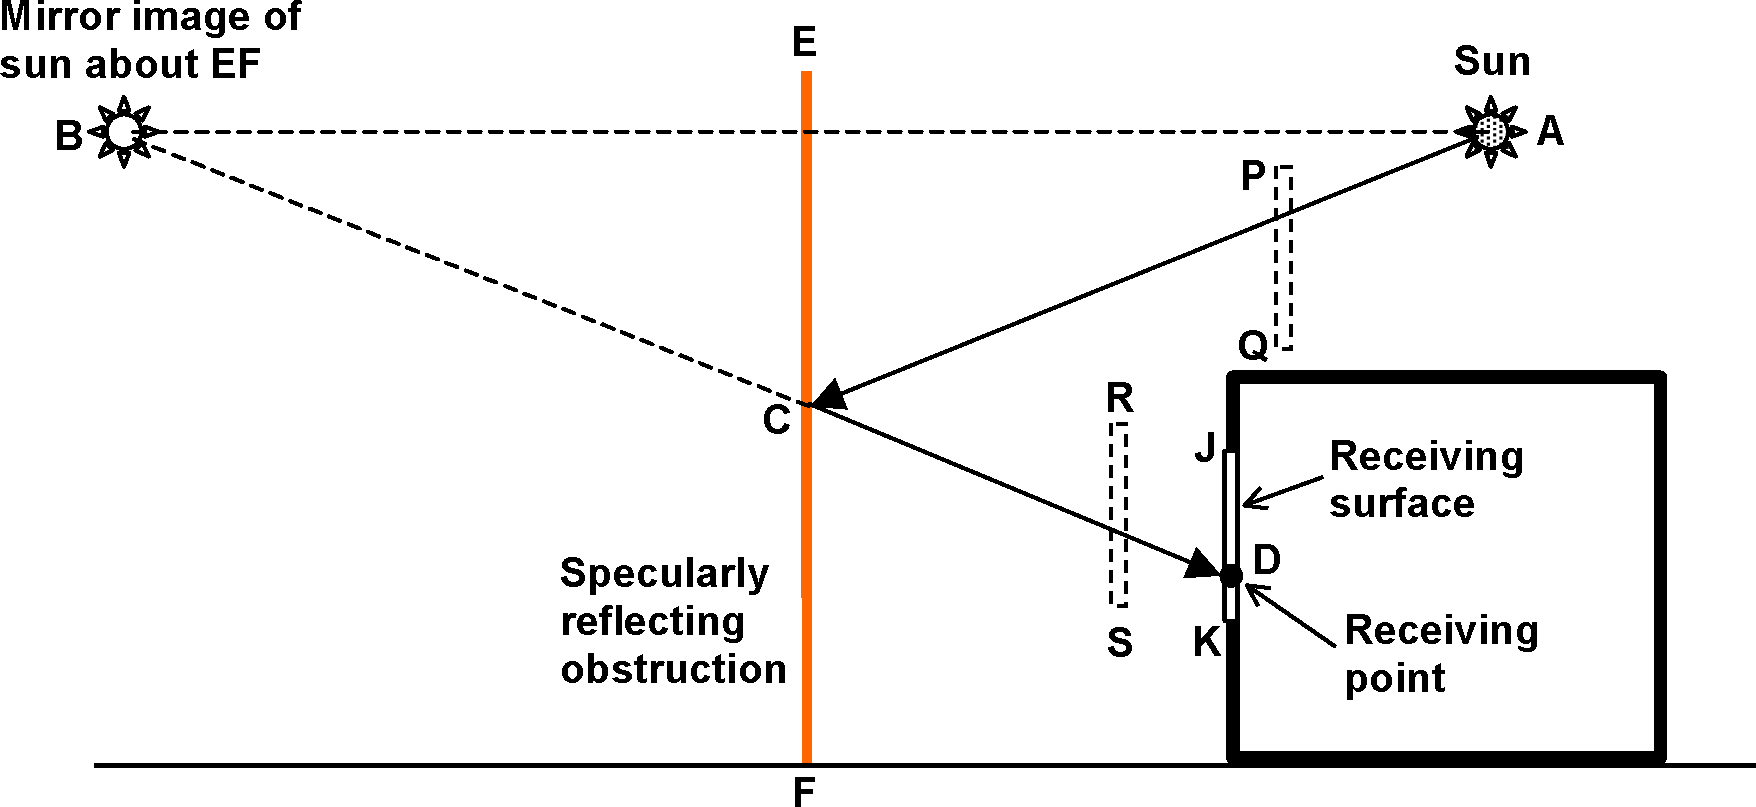
\includegraphics[width=0.9\textwidth, height=0.9\textheight, keepaspectratio=true]{media/image703.png}
\caption{Two-dimensional schematic showing specular reflection from an obstruction such as the glazed façade of a neighboring building. The receiving point receives specularly reflected beam solar radiation if (1) DB passes through specularly reflecting surface EF, (2) CD does not hit any obstructions (such as RS), and (3) AC does not hit any obstructions (such as PQ). \protect \label{fig:two-dimensional-schematic-showing-specular}}
\end{figure}

The calculation procedure is as follows:

1.~~~~Select receiving point D on receiving surface JK.

2.~~~~Select specularly reflecting surface EF.

3.~~~~Find the mirror image, B, of the sun with respect to the plane of EF and construct ray DB.

4.~~~~Check if DB passes through EF; if yes, find intersection point C and construct ray CD.

5.~~~~Check if CD is obstructed.

6.~~~~If no, construct ray AC and check if it is obstructed.

7.~~~~If no, find reflected beam irradiance (W/m\(^{2}\)) at D:

\begin{equation}
I_{D,refl}^{bm} = BeamSolarRad*{\rho_{spec}}({\alpha_C})\cos {\alpha_D}
\end{equation}

where

\({\alpha_C}\) = angle of incidence of beam solar at point C of the obstruction,

\({\rho_{spec}}({\alpha_C})\) = reflectance of obstruction as a function of the angle of incidence,

\({\alpha_D}\) = angle of incidence of ray CD on JK.

The factor for specular reflection of beam solar from obstruction onto a receiving surface is calculated in subroutine CalcBeamSolSpecularReflFactors. It is given by:

\begin{equation}
{\rm{ReflFacBmToBmSolObs(RecSurfNum,IHr) }} = \sum\limits_{\scriptstyle \substack{specularly \, reflecting \, surfaces}} \left[ {\frac{1}{{{N_{rec}}}}\sum\limits_1^{{N_{rec}}} {{f_{C,glazed}}{\rho_{spec}}({\alpha_C})\cos {\alpha_D}} } \right]
\end{equation}

The program assumes that specular reflection from a surface is due to glazing. If the reflecting surface is a window belonging to the building itself (as in Figure~\ref{fig:solar-reflection-from-building-surfaces-onto}), then \({f_{C,glazed}}\) is the fraction of the window that is glazed (which is 1.0 unless the window has dividers).

If the surface is a shading surface (that represents, for example, the glazed façade of a neigboring building) the surface reflection information is entered with the Shading Surface Reflectance object. This object contains values for:

1.~~~~Diffuse solar reflectance of the unglazed part of the shading surface

2.~~~~Diffuse visible reflectance of the unglazed part of the shading surface

3.~~~~Fraction of shading surface that is glazed

4.~~~~Name of glazing construction

In this case \({f_{C,glazed}}\) is ``Fraction of shading surface that is glazed'' and \({\rho_{spec}}({\alpha_C})\) is the front reflectance of the indicated glazing construction as a function of beam solar incidence angle.

The above specular reflection factor is used in the timestep calculation to find the beam irradiance on a receiving surface due to beam-beam reflection from obstructions:

\begin{equation}
QRadSWOutIncBmToBmReflObsRecSurfNum) = BeamSolarRad * (WeightNow * ReflFacBmToBmSolObs(RecSurfNum,HourOfDay) + WeightPreviousHour * ReflFacBmToBmSolObs(RecSurfNum,PreviousHour))
\end{equation}
